\documentclass[dutch]{hu}
\usepackage{apa}
\usepackage{makecell}
\usepackage{longtable}
\usepackage{makeidx}
\usepackage{pdfpages}
\usepackage{hyperref}
\usepackage{graphicx}
\usepackage{pdflscape}
% \date{4 december 2015}
% \addbibresource{literatuur.bib}
\makeindex
\title{TH06 Team 12}

\author{Christiaan}{van den Berg}{1660475}
\author{Aydin}{Biber}{1666849}
\author{Martijn}{van Dijk}{1660713}
\author{Chiel}{Douwes}{1666311}

\teacher{Wouter}{van Ooijen}
\teacher{Joost}{Schalken}
\teacher{Marten}{Wensink}
\teacher{Jan}{Zuurbier}
\subtitle{Requirements Architecture}
\begin{document}

\maketitle

\tableofcontents{}

\chapter{Functional Requirements}
\section{Inleiding}
In dit hoofdstuk zullen de use-cases worden beschreven.
Wanneer er wordt gerefereerd naar een "gebruiker" dan wordt hiermee de klant bedoelt die de wasmachine gekocht heeft en deze gebruikt om de was mee te doen.
Een "beheerder" is iemand die werkt voor het bedrijf die wasmachine's levert en beheert.
\newpage
\section{Useage Model}
\scalebox{0.7}{
  
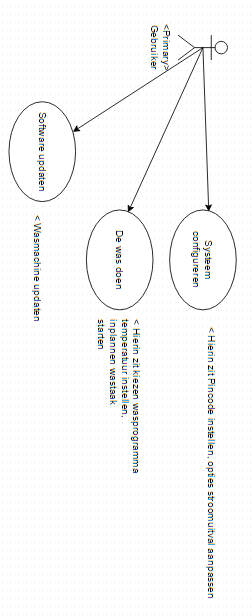
\includegraphics{usage1.png}
}

  


\section{Use Case Beschrijvingen}

\subsection{Systeem configureren}
\begin{center}
  \begin{tabular}{ | p{4cm} | p{8.5cm} | }    \hline
    Doel & Het aanpassen van de pincode of veranderen wat er gebeurt na het uitvallen van de wasmachine. \\ \hline
    Pre-condities & De gebruiker is ingelogd op de webinterface. \\ \hline
    Post-condities & De aangepaste instellingen zijn opgeslagen. \\ \hline
    Uitzonderingen & \\
    \hline
  \end{tabular}
\end{center}

\subsection{De was doen}
\begin{center}
  \begin{tabular}{ | p{4cm} | p{8.5cm} | }    \hline
    Doel & Zorgen dat de was gewassen wordt. \\ \hline
    Pre-condities & De gebruiker is ingelogd op de webinterface. \\ \hline
    Post-condities & De wasmachine is een wastaak aan het uitvoeren. \\ \hline
    Uitzonderingen & \\
    \hline
  \end{tabular}
\end{center}

\subsection{Authenticeren}
\begin{center}
  \begin{tabular}{ | p{4cm} | p{8.5cm} | } \hline
  Doel & Vaststellen dat degene die probeert toegang te krijgen tot de webinterface daadwerkelijk bevoegd is om de wasmachine te bedienen. \\ \hline
  Pre-condities & Er is een webinterface-sessie gestart.\\ \hline
  Post-condities & De gebruiker is geauthenticeerd. \\ \hline
  Uitzonderingen & De gebruiker sluit de browser. De wasmachine gaat verder met taken indien deze voor het sluiten waren doorgegeven. \\
  \end{tabular}
\end{center}

\subsection{Software updaten}
\begin{center}
  \begin{tabular}{ | p{4cm} | p{8.5cm} | }    \hline
    Doel & Het ontvangen van een update door deze te accepteren. \\ \hline
    Pre-condities & De gebruiker is ingelogd op de webinterface. \\ \hline
    Post-condities & Een nieuw wasprogramma is toegevoegd aan de lijst van wasprogramma's. \\ \hline
    Uitzonderingen &  \\
    \hline
  \end{tabular}
\end{center}

\subsection{Log inzien}
\begin{center}
  \begin{tabular}{ | p{4cm} | p{8.5cm} | }    \hline
    Doel & Het lezen van het logbestand om informatie te kunnen achterhalen over het systeem. \\ \hline
    Pre-condities & \\ \hline
    Post-condities & \\ \hline
    Uitzonderingen &  \\
    \hline
  \end{tabular}
\end{center}

\subsection{Hervatten wasprogramma}
\begin{center}
  \begin{tabular}{ | p{4cm} | p{8.5cm} | }    \hline
    Doel & Het hervatten van het huidige wasprogramma na een stroomstoring. \\ \hline
    Pre-condities & Er is een stroomstoring geweest waardoor het systeem tijdelijk niet in staat was om het wasprogramma uit te voeren. \\ \hline
    Post-condities & Het systeem is bezit met het uitvoeren van het wasprogramma vanaf het laatst bereikte punt. \\ \hline
    Uitzonderingen & De gebruiker heeft bij de instellingen aangegeven niet het programma te willen hervatten na een storing maar dat deze moet worden stopgezet. Het systeem pompt het water weg en ontgrendelt de deur. \\
    \hline
  \end{tabular}
\end{center}

\section{Activity Diagrams}
\subsection{De was doen}
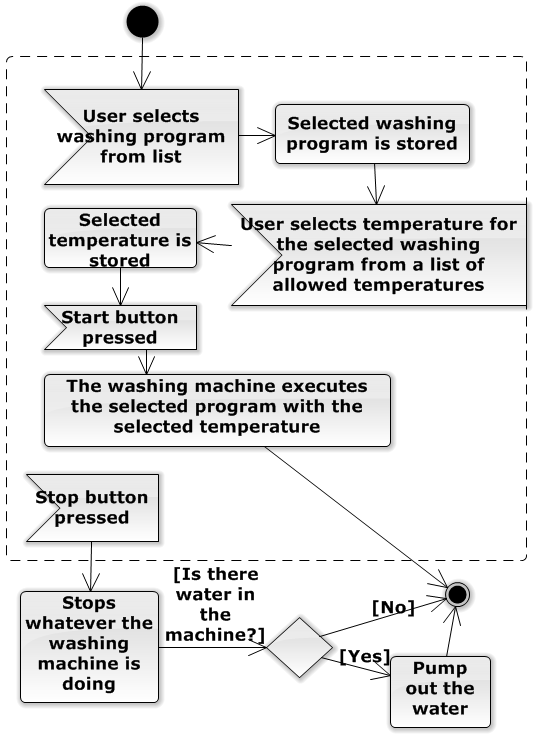
\includegraphics{wasActivity.png}

\subsection{Systeem configureren}
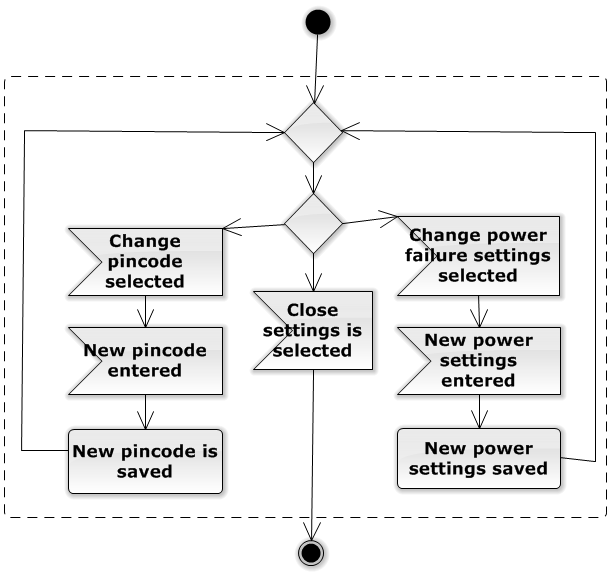
\includegraphics{configureActivity.png}

\subsection{Software updaten}
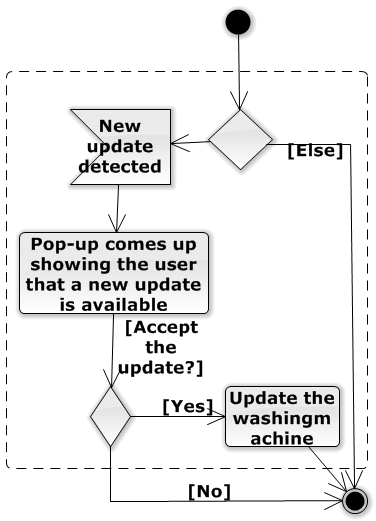
\includegraphics{updateActivity.png}

\subsection{Inloggen}
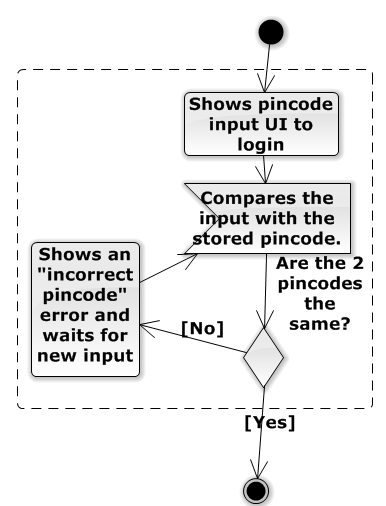
\includegraphics{loginActivity.png}

\chapter{Non-Functional Requirements}

\printbibliography

\end{document}